% section2_2_prior.tex — Module B: Bo
% Addresses QHM Core Task 1, §3.1 (likelihood) and §3.2 (prior).
\subsection{Likelihood and Prior}\label{sec:prior}

\paragraph{Likelihood (Core Task~1, §3.1)}

Let $y_i$ denote the daily rental count and let $x_{i1},x_{i2}\in[0,1]$ denote the min--max normalised temperature and humidity for observation $i=1,\dots,n$ with $n=360$. The empirical distribution of $y$ is approximately symmetric with sample mean $\bar{y}=4392$, sample standard deviation $s_y=1936$, and range $[22,\,8555]$. We adopt a homoscedastic Gaussian linear regression as the sampling model:
\begin{equation}
y_i \mid \boldsymbol{\beta},\sigma \;\stackrel{\text{ind}}{\sim}\; \mathcal{N}\!\bigl(\mu_i,\,\sigma^{2}\bigr),
\qquad
\mu_i \;=\; \beta_0 + \beta_1\,x_{i1} + \beta_2\,x_{i2},
\qquad
\boldsymbol{\beta}=(\beta_0,\beta_1,\beta_2)^{\!\top}.
\label{eq:likelihood}
\end{equation}

Two natural alternatives were considered and rejected. A Poisson likelihood imposes equidispersion ($\operatorname{Var}=\operatorname{\mathbb{E}}$); the empirical variance-to-mean ratio of $y$ exceeds unity by an order of magnitude, so a Poisson specification would yield artificially narrow credible intervals. A Negative Binomial likelihood relaxes this constraint via an extra dispersion parameter but introduces a non-Gaussian link without a corresponding gain in fit, given the approximate symmetry of $y$. The Gaussian specification~\eqref{eq:likelihood} is therefore preferred and the Negative Binomial is retained as a robustness-check candidate.

\paragraph{Prior specification (Core Task~1, §3.2)}

We assign mutually independent weakly informative priors,
\begin{equation}
\beta_j \;\sim\; \mathcal{N}\!\bigl(0,\,\tau_\beta^{2}\bigr),\quad j=0,1,2,
\qquad
\sigma \;\sim\; \mathrm{Half\text{-}}\mathcal{N}\!\bigl(\tau_\sigma\bigr),
\label{eq:priors}
\end{equation}
with hyperparameters $\tau_\beta = 10{,}000$ and $\tau_\sigma = 3{,}000$. Under~\eqref{eq:priors} each $\beta_j$ has prior mean, median, and mode equal to zero, prior standard deviation $\tau_\beta$, and 95\% prior credible interval $\approx(-19{,}600,\,19{,}600)$. The Half-Normal prior on $\sigma$ enforces the positivity constraint $\sigma>0$ and yields the closed-form summaries $\operatorname{\mathbb{E}}[\sigma]=\tau_\sigma\sqrt{2/\pi}\approx 2394$, $\operatorname{SD}(\sigma)=\tau_\sigma\sqrt{1-2/\pi}\approx 1808$, prior median $\tau_\sigma\Phi^{-1}(0.75)\approx 2024$, and 95-th percentile $\approx 5880$ (Table~\ref{tab:priors}).

\begin{table}[htbp]
\centering\small
\caption{Prior distributions and implied measures of location and dispersion.}
\label{tab:priors}
\begin{tabular}{lllcc}
\hline
Parameter & Distribution & Hyperparameter(s) & Prior mean & Prior SD \\
\hline
$\beta_0,\beta_1,\beta_2$ & Normal      & $\tau_\beta = 10{,}000$ & $0$            & $10{,}000$ \\
$\sigma$                  & Half-Normal & $\tau_\sigma = 3{,}000$ & $\approx 2394$ & $\approx 1808$ \\
\hline
\end{tabular}
\end{table}

\paragraph{Calibration of hyperparameters}

Both hyperparameters are calibrated on the empirical scale of the data. Since each $x_{ij}$ is normalised to $[0,1]$, a unit change in covariate $j$ corresponds to its full empirical range, and plausible coefficient magnitudes are bounded above by $\max_i y_i-\min_i y_i\approx 8.5\times 10^{3}$. Setting $\tau_\beta=10{,}000$ places approximately 95\% of prior mass on $|\beta_j|<19{,}600$, enveloping the ordinary-least-squares (OLS) estimates $(\hat\beta_0,\hat\beta_1,\hat\beta_2)\approx(2548,\,6796,\,-2370)$ while excluding only values that would imply effects exceeding the empirical range of $y$. The choice $\tau_\sigma=3{,}000$ aligns the prior median for $\sigma$ ($\approx 2024$) with the empirical scale $s_y\approx 1936$, accommodates the OLS residual standard error $\hat\sigma_{\text{OLS}}=1497$ in a region of substantial prior mass, and avoids the small-scale pathologies of the Inverse-Gamma. By design, $\tau_\beta$ and $\tau_\sigma$ are an order of magnitude larger than the posterior standard deviations reported in Section~\ref{sec:posterior}, so the likelihood dominates the posterior and Section~\ref{sec:sensitivity} can meaningfully assess sensitivity to the prior.

\paragraph{Prior predictive check}

To verify that~\eqref{eq:priors} is reasonable on the natural scale of the response, we drew $500$ samples from the joint prior predictive distribution of $y$ (Figure~\ref{fig:prior_pred}). The resulting distribution is approximately symmetric about zero and spans roughly $\pm 30{,}000$ — about seven times the empirical range — confirming the weakly informative character of the specification. A portion of prior mass falls below zero, which is physically inadmissible but acceptable as an artefact of unconstrained Gaussian priors on $\boldsymbol{\beta}$; this region carries negligible posterior probability once the data are conditioned on.

\begin{figure}[htbp]
\centering
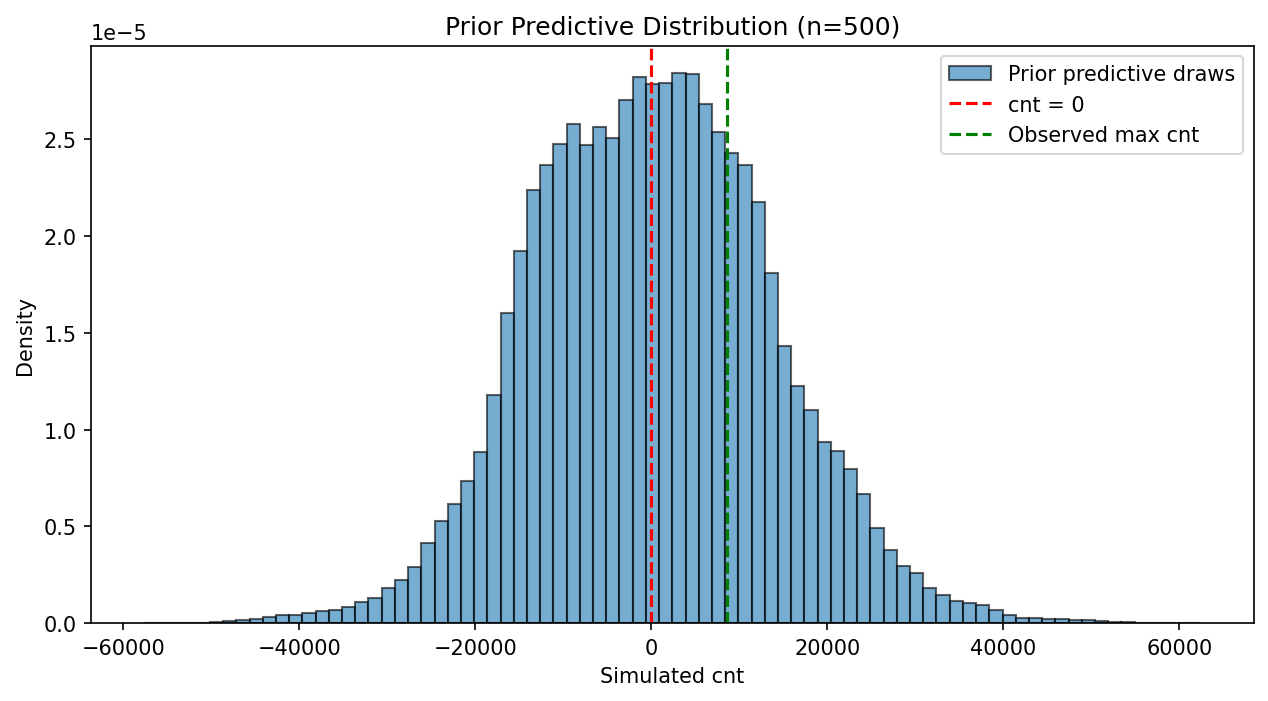
\includegraphics[width=0.55\textwidth]{../results/figures/prior_predictive.png}
\caption{Prior predictive distribution of $y$ from $500$ joint-prior draws. Dashed lines mark $y=0$ and the maximum observed value $8555$.}
\label{fig:prior_pred}
\end{figure}
